\chapter{Two Dimensional Deterministic Case}\label{chap:twod-deterministic}

In two dimensions, with deterministic coefficients Laplace's equation takes the
following form:

\begin{equation}\label{eq:two-d-deterministic}
\begin{aligned}
    -\nabla\cdot(a\nabla u(\v{x})) + \v{b} \cdot \nabla u(\v{x}) + c u(\v{x}) &= f(\v{x})
                               &\text{ in } D = [0,1] \times [0,1] \\
    u(\v{x}) &= g(\v{x}) &\text{ on } \partial D = \Gamma
\end{aligned}
\end{equation}

where $a, c \in \mathbb{R}$, $\v{b} \in \mathbb{R}^2$ and $f, g \in L^2(D)$ are
given. In our case we will choose $g(\v{x}) = 0$ to impose a Dirichlet boundary
condition on the problem

\section{Weak Formulation}

\todo[inline]{Give proper definitions of the trial and test spaces}

As with the one dimensional case, the first step in implementing the finite
element method for this problem is to obtain the weak formulation of the above
equation. Which involves multiplying through by $v \in W$ and integrating over
the domain:

\begin{equation}
    -\int_{D}{v(\nabla\cdot(a\nabla{u}))}\,dD +
    -\int_{D}\v{b}\cdot v\nabla{u}\,dD +
    c\int_{D}uv\,dD = \int_{D}fv\,dD
\end{equation}

Applying Green's first integral identity to the first term we get:

\begin{equation}
    \int_{D}v(\nabla\cdot(a\nabla u))\, dD =
    -a\int_{\Gamma}\underbrace{v\frac{\partial{u}}{\partial{n}}}_{ =0} \,d\Gamma
    + a\int_{D}\nabla{v}\cdot\nabla{u}\,dD
\end{equation}

where the underbraced integrand is zero on the boundary as $v \in W$ it
vanishes on the boundary. Thus the continuous weak formulation is given by:

\begin{equation}\label{eq:wk-twod-deterministic}
    a\int_{D}\nabla{v}\cdot\nabla{u}\,dD +
    \int_{D}\v{b}\cdot v\nabla{u}\,dD + c\int_{D}uv\,dD =
    \int_{D}fv\,dD
\end{equation}

where we need to find $u \in V$ such that \myref{eq:wk-twod-deterministic}
holds $\forall v \in W$

\section{Discrete Formulation}

\todo[inline]{This probably needs some work, especially when it comes to indices etc.}

Moving from the one dimensional case to two dimensions suddenly adds a number
of considerations since, unlike the one dimensional interval any two
dimensional domain can come in a wide array of shapes. Therefore the method of
discretisation must be chosen with the shape of the domain in mind, as what may
be suitable for one domain would fail to capture certain features of
another.However as the focus of this project is not on finding a discretisation
for arbitrary domains, we have chosen the unit square since a simple uniform
triangulation will be sufficient.

Given a parameter $N \in \mathbb{N}$ we start with square grid with spacing $h
= 1/N$ then at each of the $M: = (N+1)^2$ intersections we place a node $x_i$,
$i \in \{0,\ldots,M\}$. Then we split each grid square into 2 triangles
using the diagonal of negative slope, dividing the domain into triangular
elements $T_k$ which we can then use to define the discretisation:

\[
    \mathcal{T}_h = \bigcup_{k=1}^{2N^2} T_k
\]

See Figure \ref{fig:two-d-discretisation} for an example of such a
discretisation.

\begin{figure}
\centering
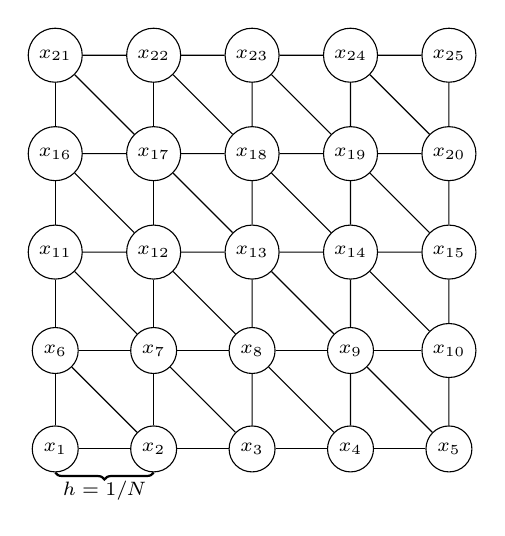
\begin{tikzpicture}[scale=5]

    \scriptsize
    % Place each of the nodes in the grid
    % First the boundary nodes

    % Place the nodes
    \foreach \x in {0,...,4}
        \foreach \y in {0,...,4}
    {
         \pgfmathtruncatemacro{\idx}{\y*5 + (\x + 1)}
         \node[circle,draw=black]
            (\x\y) at (0.25*\x,0.25*\y) {$x_{\idx}$};
    }

    % Next, the horizontal grid lines
    \foreach \y in {0,...,4}
       \foreach \x in {0,...,3}
    {
        \pgfmathtruncatemacro{\idx}{\x + 1}
        \draw (\x\y) -- (\idx\y);
    }

    % Now for the verticals
    \foreach \x in {0,...,4}
        \foreach \y in {0,...,3}
    {
        \pgfmathtruncatemacro{\idx}{\y + 1}
        \draw(\x\y) -- (\x\idx);
    }

    % Finally... the diagonals
    \foreach \y in {1,...,4}
        \foreach \x in {0,...,3}
    {
        \pgfmathtruncatemacro{\xidx}{\x + 1}
        \pgfmathtruncatemacro{\yidx}{\y - 1}
        \draw (\x\y) -- (\xidx\yidx);
    }

    % Bonus round, show the density of the grid
    \draw[thick,decoration={brace,mirror},decorate]
      (0,-0.06) -- (0.25, -0.06)
      node[pos=0.5,anchor=north]{$h=1/N$};
\end{tikzpicture}


\caption{Example triangulation of $D$ with $N = 4$}
\label{fig:two-d-discretisation}
\end{figure}

Using this triangulation we can now define suitable finite dimensional subspaces
of our test and trial spaces $V^h \subset V$, $W^h \subset W$:

\begin{align*}
    V^h &= \{v \in V: v \text{ is linear on } T_k,\ k \in \{1,\ldots,2N^2\},
                     v \text{ is continuous on } D\} \\
    W^h &= \{w \in W: w \text{ is linear on } T_k,\ k \in \{1,\ldots,2N^2\},
                     w \text{ is continuous on } D\}
\end{align*}

Then by choosing appropriate basis functions $\phi_i$ for the above subspaces
we will be able to approximate the solution as follows:

\begin{equation}
    u^h(\v{x}) = \sum_{j=0}^Mu_j\phi_j(\v{x})
\end{equation}

where $u_j$ will be the approximate value of the solution at the node $x_j$.
Similarly we can approximate $f(\v{x})$:

\begin{equation}
    f(x) \approx \sum_{j=0}^Mf_j\phi_j(\v{x})
\end{equation}

where $f_j = f(\v{x_j})$

\todo[inline]{Give details on errors, convergence etc!}

As in the one dimensional case, an appropriate basis would be the `hat
functions' which we can define in terms of a reference function $\Phi(\v{x})$
defined with respect to an example domain around $(0,0)$.  Consider as in
Figure \ref{fig:reference-function-domain} the domain where the function has
support, then we can write $\Phi(\v{x})$ as follows:

\begin{equation}\label{eq:two-d-ref-basis-fn}
    \Phi(\v{x}) = \left\{\begin{array}{c c}
                    1 - x - y, & \text{ in } T_1 \\
                    1 - x,       & \text{ in } T_2 \\
                    1 + y,       & \text{ in } T_3 \\
                    1 + x + y,   & \text{ in } T_4 \\
                    1 + x,       & \text{ in } T_5 \\
                    1 - y,       & \text{ in } T_6 \\
                    0,           & \text{ otherwise}
                  \end{array}\right.
\end{equation}

where $\v{x} = (x, y)$. Then we can write each basis function $\phi_i$ in our
discretised domain as $\phi_i(\v{x}) = \Phi(\v{x} - \v{x_i})$

\begin{figure}
\centering
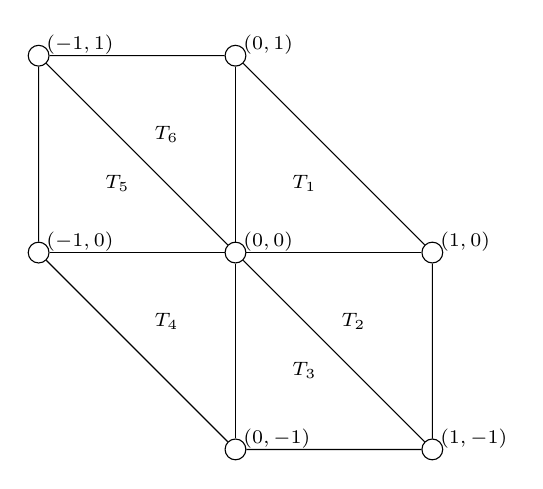
\begin{tikzpicture}[scale=2.5]
    \scriptsize

    % Place the nodes
    \node[circle,draw=black,label={[anchor=west]$(0,0)$}] (00)  at (0,0)  {};
    \node[circle,draw=black,label={[anchor=west]$(0,1)$}] (01)  at (0,1) {};
    \node[circle,draw=black,label={[anchor=west]$(1,0)$}] (10)  at (1,0)  {};
    \node[circle,draw=black,label={[anchor=west]$(-1,0)$}] (-10) at (-1,0) {};
    \node[circle,draw=black,label={[anchor=west]$(0,-1)$}] (0-1) at (0,-1) {};
    \node[circle,draw=black,label={[anchor=west]$(-1,1)$}] (-11) at (-1,1) {};
    \node[circle,draw=black,label={[anchor=west]$(1,-1)$}] (1-1) at (1,-1) {};

    % Draw the lines
    \draw (00) -- (01);
    \draw (00) -- (10);
    \draw (01) -- (10);
    \draw (00) -- (-10);
    \draw (00) -- (0-1);
    \draw (-11) -- (01);
    \draw (-11) -- (00);
    \draw (-11) -- (-10);
    \draw (-10) -- (0-1);
    \draw (0-1) -- (1-1);
    \draw (1-1) -- (10);
    \draw (00) -- (1-1);

    % Finally the T's
    \node (T1) at (0.35,0.35) {$T_1$};
    \node (T2) at (0.6, -0.35) {$T_2$};
    \node (T3) at (0.35, -0.6) {$T_3$};
    \node (T4) at (-0.35,-0.35) {$T_4$};
    \node (T5) at (-0.6, 0.35) {$T_5$};
    \node (T6) at (-0.35, 0.6) {$T_6$};

\end{tikzpicture}


\caption{The domain of the reference function $\Phi(\v{x})$}
\label{fig:reference-function-domain}
\end{figure}

Since the weak formulation \myref{eq:wk-twod-deterministic} has to hold forall
$v \in V$, in particular it has to hold for the basis functions
$\phi_i(\v{x})$, $i \in \{0,\ldots,M\}$ so by taking $v = \phi_i(\v{x})$ for
each $i \in \{0, \ldots, M\}$ and substituting our expansions for $u$ and $f$
we obtain:

\begin{align}
\begin{split}
    &a\int_{D}\nabla\phi_i(\v{x}) \cdot
                  \nabla\left(\sum_{j = 0}^Mu_j\phi_j(\v{x})\right)\, dD
    +\int_{D}\v{b}\cdot\phi_i(\v{x})\cdot
                  \nabla\left(\sum_{j = 0}^Mu_j\phi_j(\v{x})\right)\, dD \\
    &+c\int_{D}\phi_i(\v{x})
                    \left(\sum_{j = 0}^Mu_j\phi_j(\v{x})\right)\, dD =
    \int_{D}\left(\sum_{j = 0}^Mf_j\phi_j(\v{x})\right)
                 \phi_i(\v{x})\, dD
\end{split}
\end{align}

for each $i \in \{0, \ldots, M\}$ Then by the linearity of the integral and the
gradient operator this can be written as:

\begin{align}\label{eq:twod-deterministic-discrete}
  \begin{split}
    \sum_{j=0}^Mu_j
      \underbrace{\left(
         a\int_{D}\nabla\phi_i(\v{x})\cdot\nabla\phi_j(\v{x})\, dD
         + \v{b}\cdot\int_{D}\phi_i(\v{x})\cdot\nabla\phi_j(\v{x})\, dD
         +c\int_{D}\phi_i(\v{x})\phi_j(\v{x})\, dD
      \right)}_{:= A_{i,j}} = \\
    \sum_{j=0}^Mf_j
      \underbrace{\int_{D}\phi_i(\v{x})\phi_j(\v{x})}_{:= M_{i,j}}
  \end{split}
\end{align}

for $i \in \{1,\ldots,M\}$. This reduces the weak formulation
\myref{eq:wk-twod-deterministic} to a linear system $Au^h = Mf$ where as in the
one dimensional case $A$ is known as the stiffness matrix and $M$ is known as
the mass matrix. But due to the Dirichlet condition in
\myref{eq:two-d-deterministic} we already know the values of $u_j$ along the
boundary so the above reduces to:

\begin{equation}
    \sum_{j=1}^{(N-1)^2}A_{i,j}u_j =
    \sum_{j=0}^MM_{i,j}f_j
\end{equation}

for each $i \in \{1, \ldots, (N-1)^2\}$. Solving this system will give us an
approximation to the solution for \myref{eq:two-d-deterministic}.

\paragraph{Note:}

For convenience we can define the following \textit{bilinear form}:

\begin{equation}\label{eq:twod-deterministic-bilinear}
    \alpha(u,v) = a(\nabla u \cdot \nabla v) + u\v{b} \cdot \nabla v
                 + cuv
\end{equation}

which allows us to rewrite \myref{eq:twod-deterministic-discrete} as follows:

\begin{equation}
    \sum_{j = 0}^Mu_j\int_D\alpha(\phi_i,\phi_j)\, dD
        = \sum_{j = 0}^Mf_j\int_D\phi_i(\v{x})\phi_j(\v{x})\, dD
\end{equation}

\section{Constructing the Global System}

The last thing we need to do in order to implement the finite element method
for this problem is to determine the entries of the global mass and stiffness
matrices $M$ and $A$, respectively. Since we have discretised our domain into
many triangular elements, we can consider the contribution from each element
in turn and combine them into the global system.

Consider a triangular element $T$, comprised of the nodes $\v{k_1} = (0,0)$,
$\v{k_2} = (0,1)$, and $\v{k_3} = (1,0)$ with corresponding global basis functions
$\phi_{k_1}, \phi_{k_2}, \phi_{k_3}$. Now if we compare Figure
\ref{fig:twod-local-basis}, with Figure \ref{fig:reference-function-domain}
we see that the dashed lines denote the support of each of the basis functions
and the solid lines denote the subset of the domain which contains the triangular
element $T$.

Comparing further the two Figures we see that the triangular element $T$
corresponds to $T_1$ in the reference function for the basis function $\phi_{k1}$
and $T_5$ for $\phi_{k_2}$ and $T_3$ for $\phi_{k_3}$. This means locally in the
element $T_k$ we can define the following local basis functions:

\begin{align}\label{eq:twod-local-basis}
    \begin{split}
        \psi_1(x, y) = \Phi(\v{x} - \v{k_1})|_{T_1} &= 1 - x - y \\
        \psi_2(x, y) = \Phi(\v{x} - \v{k_2})|_{T_5} &= x \\
        \psi_3(x, y) = \Phi(\v{x} - \v{k_3})|_{T_3} &= y
    \end{split}
\end{align}

\begin{figure}
\centering
\begin{subfigure}[b]{0.30\textwidth}
    \centering
    \resizebox{\linewidth}{!}{\begin{tikzpicture}[scale=3]

    % Place the nodes of T_k
    \node[circle,draw=blue]  (k1) at (0,0) {\color{blue}$k_1$};
    \node (Tk) at (0.3, 0.3) {\color{blue}$T_k$};

    % Place the other nodes
    \node[circle,draw=black] (x0) at (-1,0) {};
    \node[circle,draw=black] (x1) at (0,-1) {};
    \node[circle,draw=black] (x2) at (-1,1) {};
    \node[circle,draw=black] (x3) at (1,-1) {};
    \node[circle,draw=black] (x4) at (1,0) {};
    \node[circle,draw=black] (x5) at (0,1) {};

    % Draw the triangle
    \draw[blue] (k1) -- (x5) -- (x4) --  (k1);
    \draw[dashed] (x5) -- (x2) -- (x0) -- (x1) -- (x3) -- (x4);
    \draw[dashed] (k1) -- (x0);
    \draw[dashed] (k1) -- (x1);
    \draw[dashed] (k1) -- (x2);
    \draw[dashed] (k1) -- (x3);

\end{tikzpicture}

}
\end{subfigure}
\begin{subfigure}[b]{0.30\textwidth}
    \centering
    \resizebox{\linewidth}{!}{\begin{tikzpicture}[scale=3]

    % Place the nodes of T_k
    \node[circle,draw=green]  (k2) at (0,0) {\color{green}$k_2$};
    \node (Tk) at (-0.6, 0.3) {\color{green}$T_k$};

    % Place the other nodes
    \node[circle,draw=black] (x0) at (-1,0) {};
    \node[circle,draw=black] (x1) at (0,-1) {};
    \node[circle,draw=black] (x2) at (-1,1) {};
    \node[circle,draw=black] (x3) at (1,-1) {};
    \node[circle,draw=black] (x4) at (1,0) {};
    \node[circle,draw=black] (x5) at (0,1) {};

    % Draw the triangle
    \draw[green] (k2) -- (x2) -- (x0) --  (k2);
    \draw[dashed] (x2) -- (x5) -- (x4) -- (x3) -- (x1) -- (x0);
    \draw[dashed] (k2) -- (x5);
    \draw[dashed] (k2) -- (x4);
    \draw[dashed] (k2) -- (x3);
    \draw[dashed] (k2) -- (x1);

\end{tikzpicture}

}
\end{subfigure}
\begin{subfigure}[b]{0.30\textwidth}
    \centering
    \resizebox{\linewidth}{!}{\begin{tikzpicture}[scale=3]

    % Place the nodes of T_k
    \node[circle,draw=red]  (k3) at (0,0) {\color{red}$k_3$};
    \node (Tk) at (0.3, -0.6) {\color{red}$T_k$};

    % Place the other nodes
    \node[circle,draw=black] (x0) at (-1,0) {};
    \node[circle,draw=black] (x1) at (0,-1) {};
    \node[circle,draw=black] (x2) at (-1,1) {};
    \node[circle,draw=black] (x3) at (1,-1) {};
    \node[circle,draw=black] (x4) at (1,0) {};
    \node[circle,draw=black] (x5) at (0,1) {};

    % Draw the triangle
    \draw[red] (k3) -- (x3) -- (x1) --  (k3);
    \draw[dashed] (x1) -- (x0) -- (x2) -- (x5) -- (x4) -- (x3);
    \draw[dashed] (k3) -- (x0);
    \draw[dashed] (k3) -- (x2);
    \draw[dashed] (k3) -- (x4);
    \draw[dashed] (k3) -- (x5);

\end{tikzpicture}

}
\end{subfigure}
\caption{Local contributions of the global basis functions
         $\phi_{k_1}, \phi_{k_2}, \phi_{k_3}$.}
\label{fig:twod-local-basis}
\end{figure}

This means that any $v \in V^h$ can locally in $T$ be written as:
\[
    v(\v{x}) = v(\v{k_1})\psi_1(\v{x}) + v(\v{k_2})\psi_2(\v{x}) + v(\v{k_3})\psi_3(\v{x})
\]

Furthermore, since we are using a uniform triangulation all of our triangles
are similar to this triangular element $T$ which we will now call the reference
triangle. Hence by introducing the mapping:

\begin{align*}
 \begin{array}{c c}
    \xi = \frac{x}{h} & \eta = \frac{y}{h}
 \end{array}
\end{align*}

we can map any triangular element $T_k$ in our discretisation onto the
reference triangle $T$ where $h$ represents the length of the sides of the
triangular element $T_k$. Hence we may write the local contribution of $T_k$ to
\myref{eq:twod-deterministic-discrete} as an integration around the reference
triangle $T$:

\begin{align}\label{eq:twod-deterministic-discrete-local}
    \begin{split}
    \sum_{r=1}^3\sum_{s=1}^3\underbrace{
      \left(
        ah^2\int_{T}\nabla\psi_r(\xi, \eta)\cdot\nabla\psi_s(\xi, \eta)\ d\xi d\eta
        + h^2\v{b} \cdot \int_{T}\psi_r(\xi,\eta)\cdot\nabla\psi_s(\xi,\eta)\ d\xi d\eta
        + ch^2\int_{T}\psi_r(\xi,\eta)\psi_s(\xi,\eta)\ d\xi d\eta
      \right)}_{A^{(k)}_{r,s}}u_s = \\
    \sum_{r=1}^3\sum_{s=1}^3\underbrace{\left(
        h^2\int_{T_k}\psi_r(\xi,\eta)\psi_s(\xi,\eta)\ d\xi d\eta
    \right)}_{M^{(k)}_{r,s}}f_s
    \end{split}
\end{align}

where $A^{(k)}$ and $M^{(k)}$ are the $3 \times 3$ local stiffness and mass
matrices respectively. Since evaluating their entries will involve derivatives
of the local basis functions we shall compute these now:

\begin{align}
    \begin{split}
        \nabla\psi_1(x, y) &= \left(\begin{array}{c} -1 \\ -1 \end{array}\right) \\
        \nabla\psi_2(x, y) &= \left(\begin{array}{c} 1 \\ 0 \end{array}\right) \\
        \nabla\psi_3(x, y) &= \left(\begin{array}{c} 0 \\ 1 \end{array}\right)
    \end{split}
\end{align}

\subsection{The Local Stiffness Matrix}:\label{sec:twod-deterministic-local-stiffness}

Similar to the one dimensional case, we now have an expression for the entries
of the local stiffness matrix, in terms of a number of integrals
\myref{eq:twod-deterministic-discrete-local} so we will only include a few
example cases and then present the results.

If we first consider the integral which gives the contribution from the
Laplacian:

\begin{equation*}
    ah^2\int_T\nabla\psi_r(\xi,\eta)\cdot\nabla\psi_s(\xi,\eta)\ d\xi d\eta =
    ah^2\int_T\psi_{r\xi}'\psi_{s\xi}' + \psi_{r\eta}'\psi_{s\eta}'\ d\xi d\eta
\end{equation*}

and if we take $r = 1$ and $s = 1$ then we get:

\begin{align*}
    ah^2\int_T(\psi_{i\xi}')^2 + (\psi_{1\eta}')^2\ d\xi d\eta
    &= ah^2\int_0^1\int_0^{1 - \eta}\frac{1}{h^2}((-1)^2 + (-1)^2)\ d\xi d\eta \\
    &= 2a\int_0^1\left[\xi\right]_0^{1 - \eta} \\
    &= 2a\left[\eta - \frac{\eta^2}{2}\right]_0^1 \\
    &= 2a\frac{1}{2} \\
    &= a
\end{align*}

Similarly let's consider the second integral corresponding to the gradient term,
in the case when $r = 1, s = 3$:

\begin{align*}
    h^2\int_T\psi_1(\xi,\eta)\v{b} \cdot \nabla\psi_3(\xi,\eta)\ d\xi d\eta
     &= h^2\int_0^1\int_0^{1-\eta}\frac{1}{h}(1 - \xi - \eta)
           \left(\begin{array}{c} b_1 \\b_2 \end{array}\right) \cdot
           \left(\begin{array}{c} 0 \\ 1 \end{array}\right)\ d\xi d\eta \\
     &= hb_2\int_0^1\int_0^{1-\eta} 1 - \xi - \eta \ d\xi d\eta \\
     &= hb_2\int_0^1\left[\xi - \frac{\xi^2}{2} - \eta\xi \right]_0^{1-\eta}\ d\eta \\
     &= hb_2\int_0^1(1 -\eta) - \eta(1-\eta) - \frac{(1 - \eta)^2}{2}\ d\eta \\
     &= hb_2\int_0^1\frac{1}{2} -\eta +\frac{\eta^2}{2}\ d\eta \\
     &= \left[\frac{\eta}{2} - \frac{\eta^2}{2} + \frac{\eta^3}{6}\right]_0^1 \\
     &= \frac{hb_2}{6}
\end{align*}

Now considering third integral, in the case where $r = 3, s = 2$:

\begin{align*}
    ch^2\int_T\psi_3(\xi,\eta)\psi_2(\xi,\eta)\ d\xi d\eta
    &= ch^2\int_0^1\int_0^{1-\eta}\xi\eta\ d\xi d\eta \\
    &= ch^2\int_0^1\left[\frac{\xi^2\eta}{2}\right]_0^{1-\eta}\ d\eta \\
    &= ch^2\int_0^1\frac{(1-\eta)^2\eta}{2}\ d\eta \\
    &= \frac{ch^2}{2}\left[\frac{\eta^2}{2} - \frac{2\eta^3}{3} - \frac{\eta^4}{4}\right]_0^1 \\
    &= \frac{ch^2}{24}
\end{align*}

Following a similar process for the rest of the entries gives us the following
form for the local stiffness matrix:

\begin{equation}\label{eq:twod-local-stiffness}
 A^{(k)} =
    \frac{a}{2}\left(\begin{array}{c c c}
         2 & -1 & -1 \\
        -1 &  1 &  0 \\
        -1 &  0 &  1
    \end{array}\right)
    + \frac{h}{12} \left(\begin{array}{c c c}
        -(b_1 + b_2) & 2b_1 & 2b_2 \\
        -(b_1 + b_2) & 2b_1  & 2b_2 \\
        -(b_1 + b_2) & 2b_1  & 2b_2
    \end{array}\right)
    + \frac{ch^2}{24}\left(\begin{array}{c c c}
         2 &  1 &  1 \\
         1 &  2 &  1 \\
         1 &  1 &  2
      \end{array}\right)
\end{equation}

where $a, c \in \mathbb{R}$ and $\v{b} = (b_1, b_2) \in \mathbb{R}^2$
correspond to the parameters which define the original equation
\myref{eq:two-d-deterministic} we considered.

\subsection{The Local Mass Matrix}\label{sec:twod-deterministic-local-mass}

Following the same procedure, we can also compute the entries of the local mass
matrix as defined in \myref{eq:twod-deterministic-discrete-local}, in fact the
entries of the mass matrix are the same as those in those in the third term of
the local stiffness matrix so we have already seen the case $r = 3, s = 2$ and
by the fact that the matrix is symmetric the case $r = 2, s = 3$. So let's
consider the case where $r = 1, s = 2$:

\begin{align*}
    h^2\int_T\psi_1(\xi,\eta)\psi_2(\xi,\eta)\ d\xi d\eta
    &=  h^2\int_0^1\int_0^{1-\eta}(1 - \xi -\eta)\xi\ d\xi d\eta \\
    &= h^2\int_0^1\left[\frac{\xi^2}{2} -\frac{\xi^3}{3}
                        -\frac{\xi^2\eta}{2}\right]_0^{1-\eta}\  d\eta \\
    &= h^2\int_0^1\frac{(1-\eta)^2}{2} - \frac{(1-\eta)^3}{3}- \frac{(1-\eta)^2\eta}{2}\ d\eta \\
    &= \frac{h^2}{6}\int_0^1(1- \eta)^3\ d\eta \\
    &= \frac{h^2}{6}\left[\eta -\frac{3\eta}{2} + \eta^3 - \frac{\eta^4}{4}\right]_0^1 \\
    &= \frac{h^2}{24}
\end{align*}

and by symmetry this is the same as the case $r = 2, s = 1$. Finally we can consider the case
$r = 1, s = 3$

\begin{align*}
    h_2\int_T\psi_1(\xi, \eta)\psi_3(\xi, \eta)\ d\xi d\eta
    &= h^2\int_0^1\int_0^{1-\eta}(1 - \xi - \eta)\eta\ d\xi d\eta \\
    &= h^2\int_0^1\left[\xi\eta - \frac{\xi^2\eta}{2} - \eta^2\xi\right]_0^{1-\eta}\ d\eta \\
    &= h^2\int_0^1(1-\eta)\eta - \frac{(1 - \eta)^2\eta}{2} - \eta^2(1 - \eta)\ d\eta \\
    &= \frac{h^2}{2}\int_0^1(1 - \eta)^2\eta \ d\eta \\
    &= \frac{h^2}{2}\left[\frac{\eta^2}{2} - \frac{2\eta^3}{2} + \frac{\eta^4}{4}\right]_0^1 \\
    &= \frac{h^2}{24}
\end{align*}

which again by symmetry will also give us the case where $r = 3, s = 1$. If we
follow the same procedure for the remaining diagonal elements we obtain the
following form for the local mass matrix:

\begin{equation}\label{eq:twod-local-mass}
    M^{(k)} =
    \frac{h^2}{24}\left(\begin{array}{c c c}
         2 &  1 &  1 \\
         1 &  2 &  1 \\
         1 &  1 &  2
      \end{array}\right)
\end{equation}

\subsection{Assembling the Global Stiffness Matrix}\label{sec:twod-global-stiffnes-assembly}

Now that we know the form of local stiffness matrix
\myref{eq:twod-local-stiffness} we can start to assemble the global stiffness
matrix. As in the one dimensional case, we need to take into account the
contributions each of the elements surrounding a node make to its value.

However the extra dimension does mean that there are a few more cases that we
have to consider. Firstly due to the boundary conditions on the problem only
the interior nodes are unknown - hence the fact that the global stiffness
matrix has dimension $(N - 1) \times (N - 1)$ it will be useful for us to
relabel the interior nodes to $X_k$, $k \in \{1, \ldots, (N-1)^2\}$ and let's
consider the $k$-th row of the global stiffness matrix:

\begin{align}
  \begin{split}
    A_{k,i} &= a\int_D\nabla\phi_k\cdot\nabla\phi_i\, dD
            + \v{b} \cdot \int_D\phi_k\cdot\nabla\phi_i\, dD
            + c\int_D\phi_k\phi_i\, dD \\
            &= \int_D\alpha(\phi_k,\phi_i)\, dD
  \end{split}
\end{align}

for each $i \in \{1,\ldots,(N-1)^2)\}$ and where we used the \textit{bilinear
form} we defined in \myref{eq:twod-deterministic-bilinear}. Looking at Figure
\ref{fig:twod-global-basis-contrib} we can see each of the values of $i$ where
the corresponding basis function $\phi_i$ has support in at least a subset of
the support of $\phi_k$. (Assuming that the node $X_k$ is on the interior of
the interior part of the domain).  This means the non zero entries in the
$k$-th row of $A$ are given by:

\begin{align}
  \begin{split}
      \int_D\alpha(\phi_k,\phi_k)\, dD
        &= 2\int_T\alpha(\psi_1,\psi_1)\, dT + 2\int_T\alpha(\psi_2,\psi_2)\, dT
         + 2\int_T\alpha(\psi_3,\psi_3)\, dT \\
      \int_D\alpha(\phi_k,\phi_{k+1})\, dD
          &= \int_T\alpha(\psi_1,\psi_2)\, dT + \int_T\alpha(\psi_2,\psi_1)\, dT \\
      \int_D\alpha(\phi_k,\phi_{k-1})\, dD
          &= \int_T\alpha(\psi_2,\psi_1)\, dT + \int_T\alpha(\psi_1,\psi_2)\, dT \\
      \int_D\alpha(\phi_k,\phi_{k+N})\, dD
          &= \int_T\alpha(\psi_3,\psi_1)\, dT + \int_T\alpha(\psi_1,\psi_3)\, dT \\
      \int_D\alpha(\phi_k,\phi_{k-N})\, dD
          &= \int_T\alpha(\psi_1,\psi_3)\, dT + \int_T\alpha(\psi_3,\psi_1)\, dT \\
      \int_D\alpha(\phi_k,\phi_{(k+1) - N})\, dD
          &= \int_T\alpha(\psi_2,\psi_3)\, dT + \int_T\alpha(\psi_3,\psi_2)\, dT \\
      \int_D\alpha(\phi_k,\phi_{(k-1) + N})\, dD
          &= \int_T\alpha(\psi_3,\psi_2)\, dT + \int_T\alpha(\psi_2,\psi_3)\, dT
  \end{split}
\end{align}

where again referring to Figure \ref{fig:twod-global-basis-contrib} you can see
where these basis functions share support and how they are rewritten locally in
that region with respect to the reference triangle $T$. Furthermore looking at
the definition of the local stiffness matrix \myref{eq:twod-local-stiffness}
and noting the fact that in the case of this problem and chosen discretisation
the local stiffness matrix takes the same form in each triangular element
$T_k$. Hence the non zero elements of the $k$-th row of $A$ are given by:

\begin{align}
  \begin{split}
    A_{k,k} &= 2\Ak{1}{1} + 2\Ak{2}{2} + 2\Ak{3}{3} \\
    A_{k,k+1} &= \Ak{1}{2} + \Ak{2}{1} \\
    A_{k,k-1} &= \Ak{2}{1} + \Ak{1}{2} \\
    A_{k,k+N} &= \Ak{3}{1} + \Ak{1}{3} \\
    A_{k,k-N} &= \Ak{1}{3} + \Ak{3}{1} \\
    A_{k,(k+1)-N} &= \Ak{2}{3} + \Ak{2}{3} \\
    A_{k,(k-1)+N} &= \Ak{3}{2} + \Ak{2}{3}
  \end{split}
\end{align}

\begin{figure}
    \centering
    \begin{subfigure}[b]{0.30\textwidth}
    \centering
    \resizebox{\linewidth}{!}{
        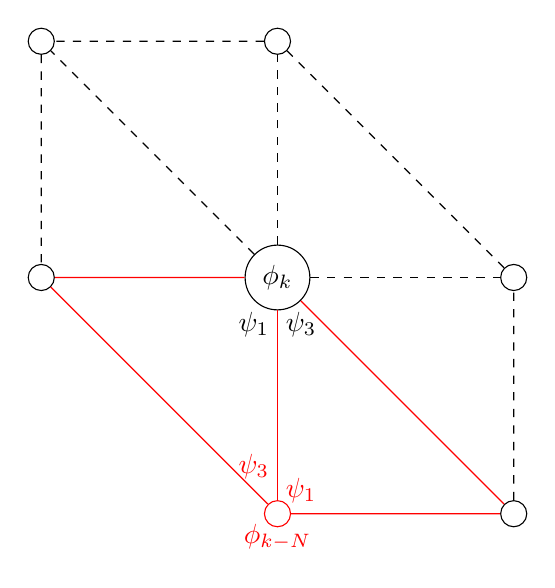
\begin{tikzpicture}[scale=3]
            % Place the center node
            \node[circle,draw=black] (k) at (0,0) {$\phi_k$};
            \node (p1) at (0.1, -0.2) {$\psi_3$};
            \node (p2) at (-0.1, -0.2) {$\psi_1$};
            \node (p2) at (-0.1, -0.8) {\color{red}$\psi_3$};
            \node (p1) at (0.1, -0.9) {\color{red}$\psi_1$};

            % Place the other nodes
            \node[circle,draw=black] (x0) at (-1,0) {};
            \node[circle,draw=red] (x1) at (0,-1) {};
            \node (k1) at (0, -1.1) {\color{red}$\phi_{k-N}$};
            \node[circle,draw=black] (x2) at (-1,1) {};
            \node[circle,draw=black] (x3) at (1,-1) {};
            \node[circle,draw=black] (x4) at (1,0) {};
            \node[circle,draw=black] (x5) at (0,1) {};

            % The lines!
            \draw[red] (k) -- (x0) -- (x1) -- (x3) -- (k);
            \draw[red] (k) -- (x1);
            \draw[dashed] (x3) -- (x4) -- (x5) -- (x2) -- (x0);
            \draw[dashed] (k) -- (x4);
            \draw[dashed] (k) -- (x5);
            \draw[dashed] (k) -- (x2);
        \end{tikzpicture}}
\end{subfigure}
\begin{subfigure}[b]{0.30\textwidth}
    \centering
    \resizebox{\linewidth}{!}{
        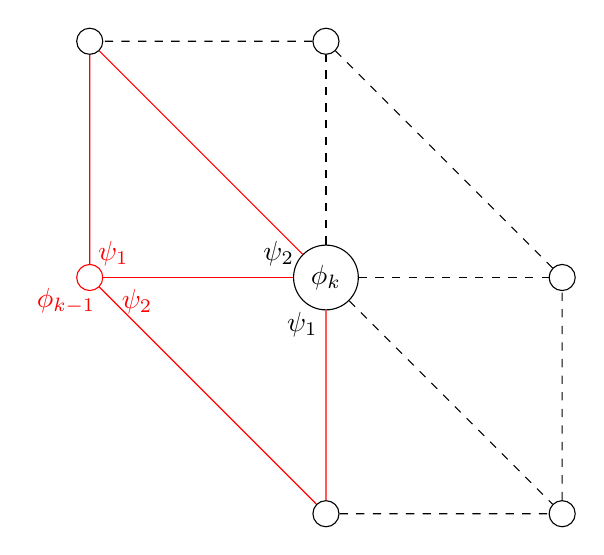
\begin{tikzpicture}[scale=3]
            % Place the center node
            \node[circle,draw=black] (k) at (0,0) {$\phi_k$};
            \node (p1) at (-0.2, 0.1) {$\psi_2$};
            \node (p2) at (-0.1, -0.2) {$\psi_1$};
            \node (p2) at (-0.8, -0.1) {\color{red}$\psi_2$};
            \node (p1) at (-0.9, 0.1) {\color{red}$\psi_1$};

            % Place the other nodes
            \node[circle,draw=red] (x0) at (-1,0) {};
            \node (k1) at (-1.1, -0.1) {\color{red}$\phi_{k-1}$};
            \node[circle,draw=black] (x1) at (0,-1) {};
            \node[circle,draw=black] (x2) at (-1,1) {};
            \node[circle,draw=black] (x3) at (1,-1) {};
            \node[circle,draw=black] (x4) at (1,0) {};
            \node[circle,draw=black] (x5) at (0,1) {};

            % The lines!
            \draw[red] (k) -- (x1) -- (x0) -- (x2) -- (k);
            \draw[red] (k) -- (x0);
            \draw[dashed] (x1) -- (x3) -- (x4) -- (x5) -- (x2);
            \draw[dashed] (k) -- (x5);
            \draw[dashed] (k) -- (x3);
            \draw[dashed] (k) -- (x4);
        \end{tikzpicture}}
\end{subfigure}
\begin{subfigure}[b]{0.30\textwidth}
    \centering
    \resizebox{\linewidth}{!}{
        \begin{tikzpicture}[scale=3]
            % Place the center node
            \node[circle,draw=black] (k) at (0,0) {$\phi_k$};
            \node (p1) at (-0.2, 0.1) {$\psi_2$};
            \node (p2) at (-0.1, 0.25) {$\psi_3$};
            \node (p2) at (-0.8, 0.9) {\color{red}$\psi_2$};
            \node (p1) at (-0.9, 0.8) {\color{red}$\psi_3$};

            % Place the other nodes
            \node[circle,draw=black] (x0) at (-1,0) {};
            \node[circle,draw=black] (x1) at (0,-1) {};
            \node[circle,draw=red] (x2) at (-1,1) {};
            \node (k1) at (-1, 1.15) {\color{red}$\phi_{(k-1) + N}$};
            \node[circle,draw=black] (x3) at (1,-1) {};
            \node[circle,draw=black] (x4) at (1,0) {};
            \node[circle,draw=black] (x5) at (0,1) {};

            % The lines!
            \draw[red] (k) -- (x5) -- (x2) -- (x0) -- (k);
            \draw[red] (k) -- (x2);
            \draw[dashed] (x0) -- (x1) -- (x3) -- (x4) -- (x5);
            \draw[dashed] (k) -- (x1);
            \draw[dashed] (k) -- (x3);
            \draw[dashed] (k) -- (x4);
        \end{tikzpicture}}
\end{subfigure}
\begin{subfigure}[b]{0.30\textwidth}
    \centering
    \resizebox{\linewidth}{!}{
        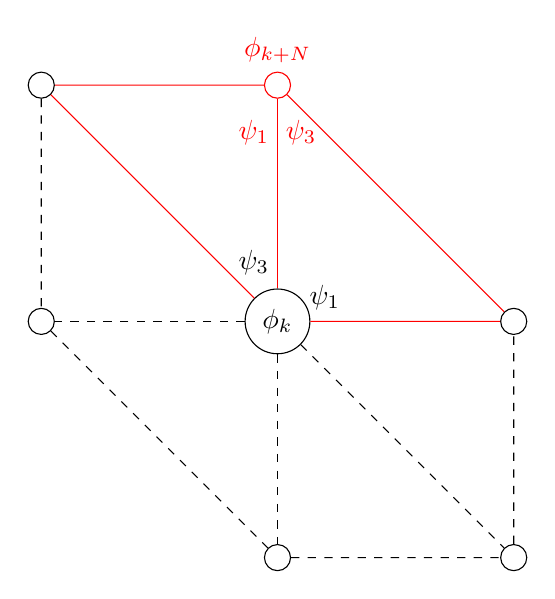
\begin{tikzpicture}[scale=3]
            % Place the center node
            \node[circle,draw=black] (k) at (0,0) {$\phi_k$};
            \node (p1) at (0.2, 0.1) {$\psi_1$};
            \node (p2) at (-0.1, 0.25) {$\psi_3$};
            \node (p2) at (0.1, 0.8) {\color{red}$\psi_3$};
            \node (p1) at (-0.1, 0.8) {\color{red}$\psi_1$};

            % Place the other nodes
            \node[circle,draw=black] (x0) at (-1,0) {};
            \node[circle,draw=black] (x1) at (0,-1) {};
            \node[circle,draw=black] (x2) at (-1,1) {};
            \node[circle,draw=black] (x3) at (1,-1) {};
            \node[circle,draw=black] (x4) at (1,0) {};
            \node[circle,draw=red] (x5) at (0,1) {};
            \node (k1) at (0, 1.15) {\color{red}$\phi_{k + N}$};

            % The lines!
            \draw[red] (k) -- (x4) -- (x5) -- (x2) -- (k);
            \draw[red] (k) -- (x5);
            \draw[dashed] (x2) -- (x0) -- (x1) -- (x3) -- (x4);
            \draw[dashed] (k) -- (x0);
            \draw[dashed] (k) -- (x1);
            \draw[dashed] (k) -- (x3);
        \end{tikzpicture}}
\end{subfigure}
\begin{subfigure}[b]{0.30\textwidth}
    \centering
    \resizebox{\linewidth}{!}{
        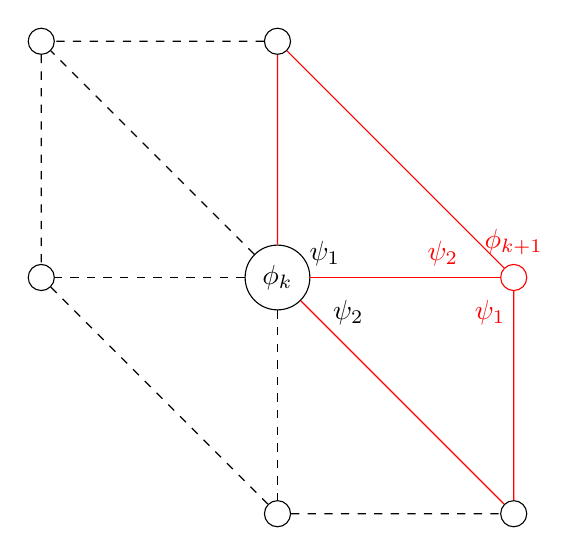
\begin{tikzpicture}[scale=3]
            % Place the center node
            \node[circle,draw=black] (k) at (0,0) {$\phi_k$};
            \node (p1) at (0.2, 0.1) {$\psi_1$};
            \node (p2) at (0.3, -0.15) {$\psi_2$};
            \node (p2) at (0.7, 0.1) {\color{red}$\psi_2$};
            \node (p1) at (0.9, -0.15) {\color{red}$\psi_1$};

            % Place the other nodes
            \node[circle,draw=black] (x0) at (-1,0) {};
            \node[circle,draw=black] (x1) at (0,-1) {};
            \node[circle,draw=black] (x2) at (-1,1) {};
            \node[circle,draw=black] (x3) at (1,-1) {};
            \node[circle,draw=red] (x4) at (1,0) {};
            \node (k1) at (1, 0.15) {\color{red}$\phi_{k+1}$};
            \node[circle,draw=black] (x5) at (0,1) {};

            % The lines!
            \draw[dashed] (x5) -- (x2) -- (x0) -- (x1) -- (x3);
            \draw[dashed] (k) -- (x2);
            \draw[dashed] (k) -- (x0);
            \draw[dashed] (k) -- (x1);
            \draw[red] (k) -- (x3) -- (x4) -- (x5) -- (k);
            \draw[red] (k) -- (x4);
        \end{tikzpicture}}
\end{subfigure}
\begin{subfigure}[b]{0.30\textwidth}
    \centering
    \resizebox{\linewidth}{!}{
        \begin{tikzpicture}[scale=3]
            % Place the center node
            \node[circle,draw=black] (k) at (0,0) {$\phi_k$};
            \node (p3) at (0.1, -0.3) {$\psi_3$};
            \node (p2) at (0.4, -0.15) {$\psi_2$};
            \node (p2) at (0.6, -0.9) {\color{red}$\psi_2$};
            \node (p3) at (0.9, -0.7) {\color{red}$\psi_3$};

            % Place the other nodes
            \node[circle,draw=black] (x0) at (-1,0) {};
            \node[circle,draw=black] (x1) at (0,-1) {};
            \node[circle,draw=black] (x2) at (-1,1) {};
            \node[circle,draw=red] (x3) at (1,-1) {};
            \node (k1) at (1, -1.1) {\color{red}$\phi_{(k + 1) - N}$};
            \node[circle,draw=black] (x4) at (1,0) {};
            \node[circle,draw=black] (x5) at (0,1) {};

            % The lines!
            \draw[dashed] (x4) -- (x5) -- (x2) -- (x0) -- (x1);
            \draw[dashed] (k) -- (x5);
            \draw[dashed] (k) -- (x2);
            \draw[dashed] (k) -- (x0);
            \draw[red] (k) -- (x1) -- (x3) -- (x4) -- (k);
            \draw[red] (k) -- (x3);
        \end{tikzpicture}}
\end{subfigure}
\begin{subfigure}[b]{0.30\textwidth}
    \centering
    \resizebox{\linewidth}{!}{
        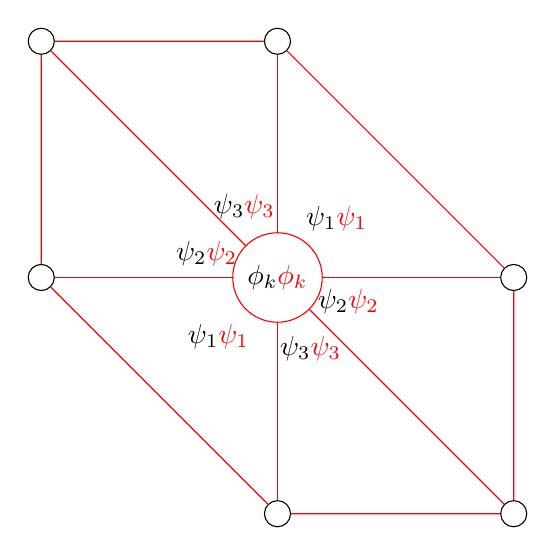
\begin{tikzpicture}[scale=3]
            % Place the center node
            \node[circle,draw=red] (k) at (0,0) {$\phi_k
                                                  \color{red}\phi_k$};
            \node (p1) at (0.14, -0.3){$\psi_3\color{red}\psi_3$};
            \node (p4) at (-0.14, 0.3) {$\psi_3\color{red}\psi_3$};
            \node (p2) at (-0.25, -0.25) {$\psi_1\color{red}\psi_1$};
            \node (p3) at (0.25, 0.25) {$\psi_1\color{red}\psi_1$};
            \node (p5) at (0.3, -0.1) {$\psi_2\color{red}\psi_2$};
            \node (p6) at (-0.3, 0.1) {$\psi_2\color{red}\psi_2$};

            % Place the other nodes
            \node[circle,draw=black] (x0) at (-1,0) {};
            \node[circle,draw=black] (x1) at (0,-1) {};
            \node[circle,draw=black] (x2) at (-1,1) {};
            \node[circle,draw=black] (x3) at (1,-1) {};
            \node[circle,draw=black] (x4) at (1,0) {};
            \node[circle,draw=black] (x5) at (0,1) {};

            % The lines!
            \draw[red] (x0) -- (x1) -- (x3) -- (x4) -- (x5) -- (x2) -- (x0);
            \draw[red] (k) -- (x0);
            \draw[red] (k) -- (x1);
            \draw[red] (k) -- (x2);
            \draw[red] (k) -- (x3);
            \draw[red] (k) -- (x4);
            \draw[red] (k) -- (x5);
        \end{tikzpicture}}
\end{subfigure}

    \caption{The contributions from the surrounding basis functions to the
        value at the node $x_k$}
    \label{fig:twod-global-basis-contrib}
\end{figure}

\paragraph{Note:}

The above only applies to nodes on the interior of the interior region - that
is nodes that are surrounded by other interior nodes. In the case of nodes on
the edge of this region their support intersects the support of nodes that are
known. In the case of these nodes the corresponding entry of the stiffness
matrix is set to zero and the value of the boundary node is taken to the right
hand side of the equation.

Let's consider an example, in the case where $N = 4$ - like in Figure
\ref{fig:two-d-discretisation} and take $a = 1, \v{b} = \v{0}, c = 0$
then the local stiffness matrix as given in
\myref{eq:twod-local-stiffness} will be given by:

\begin{equation}
    A^{(k)} = \frac{1}{2}\left[\begin{array}{c c c}
            2 & -1 & -1 \\ -1 & 1 & 0 \\ -1 & 0 & 1
    \end{array}\right]
\end{equation}

hence the non zero $i$-th entries of the $k$-th row will of the global
stiffness matrix are given by:

\begin{align}
  \begin{split}
    A_{k,k} &= \frac{2}{2}(2 + 1 + 1) = 4 \\
    A_{k,k+1} &= \frac{1}{2}(-1 -1) = -1 \\
    A_{k,k-1} &= \frac{1}{2}(-1 -1) = -1  \\
    A_{k,k+N} &= \frac{1}{2}(-1 -1) = -1 \\
    A_{k,k-N} &= \frac{1}{2}(-1 -1) = -1 \\
    A_{k,(k+1)-N} &= \frac{1}{2}(0 + 0) = 0 \\
    A_{k,(k-1)+N} &= \frac{1}{2}(0 + 0) = 0
  \end{split}
\end{align}

Therefore in this case the global stiffness matrix will be
$9 \times 9$ and take the following form:

\begin{equation}
    A = \left[\begin{array}{r r r r r r r r r}
        4 & -1 &  0 & -1 &  0 &  0 &  0 &  0 &  0 \\
       -1 &  4 & -1 &  0 & -1 &  0 &  0 &  0 &  0 \\
        0 & -1 &  4 &  0 &  0 & -1 &  0 &  0 &  0 \\
       -1 &  0 &  0 &  4 & -1 &  0 & -1 &  0 &  0 \\
        0 & -1 &  0 & -1 &  4 & -1 &  0 & -1 &  0 \\
        0 &  0 & -1 &  0 & -1 &  4 &  0 &  0 & -1 \\
        0 &  0 &  0 & -1 &  0 &  0 &  4 & -1 &  0 \\
        0 &  0 &  0 &  0 & -1 &  0 & -1 &  4 & -1 \\
        0 &  0 &  0 &  0 &  0 & -1 &  0 & -1 & 4
    \end{array}\right]
\end{equation}

\subsection{Assembling the Global Mass Matrix}

By following a similar argument to the case for the stiffness matrix and
considering Figure \ref{fig:two-d-discretisation} we find that the non zero
$i$-th entries of the $k$-th row are given by:

\begin{align}
  \begin{split}
    M_{k,k} &= 2\Mk{1}{1} + 2\Mk{2}{2} + 2\Mk{3}{3} \\
    M_{k,k+1} &= \Mk{1}{2} + \Mk{2}{1} \\
    M_{k,k-1} &= \Mk{2}{1} + \Mk{1}{2} \\
    M_{k,k+N} &= \Mk{3}{1} + \Mk{1}{3} \\
    M_{k,k-N} &= \Mk{1}{3} + \Mk{3}{1} \\
    M_{k,(k+1)-N} &= \Mk{2}{3} + \Mk{2}{3} \\
    M_{k,(k-1)+N} &= \Mk{3}{2} + \Mk{2}{3}
  \end{split}
\end{align}

So continuing the example we had in Section
\ref{sec:twod-global-stiffnes-assembly} with $N = 4 \rightarrow h = 1/4$ and
$a = 1, \v{b} = 0, c = 0$ then the local mass matrix as defined in
\myref{eq:twod-local-mass} is given by:

\begin{equation}\label{eq:twod-local-mass}
    M^{(k)} =
    \frac{1}{384}\left(\begin{array}{c c c}
         2 &  1 &  1 \\
         1 &  2 &  1 \\
         1 &  1 &  2
      \end{array}\right)
\end{equation}

hence the non zero $i$-th entries of the $k$-th row are given by:

\begin{align}
  \begin{split}
    M_{k,k} &= \frac{2}{384}(2 + 2 + 2) = \frac{12}{384}\\
    M_{k,k+1} &= \frac{1}{384}(1 + 1) = \frac{2}{384} \\
    M_{k,k-1} &= \frac{1}{384}(1 + 1) = \frac{2}{384} \\
    M_{k,k+N} &= \frac{1}{384}(1 + 1) = \frac{2}{384} \\
    M_{k,k-N} &= \frac{1}{384}(1 + 1) = \frac{2}{384} \\
    M_{k,(k+1)-N} &= \frac{1}{384}(1 + 1) = \frac{2}{384} \\
    M_{k,(k-1)+N} &= \frac{1}{384}(1 + 1) = \frac{2}{384}
  \end{split}
\end{align}

Therefore in this case the global mass matrix will be a $9 \times 25$ matrix of
the following form:

\begin{equation}
    M = \frac{1}{384}
        \left[\begin{array}{c c c c c c c c c c c c c c c c c c c c c c c c c}
    0 & 2 & 2 & 0 & 0 & 2 & 12 & 2 & 0 & 0 & 2 & 2 & 0 & 0 & 0 & 0 & 0 & 0 & 0 & 0 & 0 & 0 & 0 & 0 & 0 \\
    0 & 0 & 2 & 2 & 0 & 0 & 2 & 12 & 2 & 0 & 0 & 2 & 2 & 0 & 0 & 0 & 0 & 0 & 0 & 0 & 0 & 0 & 0 & 0 & 0 \\
    0 & 0 & 0 & 2 & 2 & 0 & 0 & 2 & 12 & 2 & 0 & 0 & 2 & 2 & 0 & 0 & 0 & 0 & 0 & 0 & 0 & 0 & 0 & 0 & 0 \\
    0 & 0 & 0 & 0 & 0 & 0 & 2 & 2 & 0 & 0 & 2 & 12 & 2 & 0 & 0 & 2 & 2 & 0 & 0 & 0 & 0 & 0 & 0 & 0 & 0 \\
    0 & 0 & 0 & 0 & 0 & 0 & 0 & 2 & 2 & 0 & 0 & 2 & 12 & 2 & 0 & 0 & 2 & 2 & 0 & 0 & 0 & 0 & 0 & 0 & 0 \\
    0 & 0 & 0 & 0 & 0 & 0 & 0 & 0 & 2 & 2 & 0 & 0 & 2 & 12 & 2 & 0 & 0 & 2 & 2 & 0 & 0 & 0 & 0 & 0 & 0 \\
    0 & 0 & 0 & 0 & 0 & 0 & 0 & 0 & 0 & 0 & 0 & 2 & 2 & 0 & 0 & 2 & 12 & 2 & 0 & 0 & 2 & 2 & 0 & 0 & 0 \\
    0 & 0 & 0 & 0 & 0 & 0 & 0 & 0 & 0 & 0 & 0 & 0 & 2 & 2 & 0 & 0 & 2 & 12 & 2 & 0 & 0 & 2 & 2 & 0 & 0 \\
    0 & 0 & 0 & 0 & 0 & 0 & 0 & 0 & 0 & 0 & 0 & 0 & 0 & 2 & 2 & 0 & 0 & 2 & 12 & 2 & 0 & 0 & 2 & 2 & 0
    \end{array}\right]
\end{equation}

\section{Example Problems and Results}

Just as in Chapter \ref{chap:oned-deterministic} to construct and solve these
linear systems we will have to make use of a computer. However in this case the
linear systems as discussed above \myref{eq:twod-deterministic-discrete} grow
on the order of $O(N^4)$ as opposed to $O(N^2)$ in the one dimensional case. In
order to handle the much greater computational complexity of these systems the
use of the Numpy linear algebra library has been replaced with the very similar
sparse section of the Scipy library \cite{scipy}.

The use of sparse matrices means memory usage and CPU time can be greatly
reduced allowing the us to handle these larger systems with relative ease. All
problems in this section have been solved using the code in Listing
\ref{code:twod-deterministic}. As with the one dimensional case the results
have been visualised with the Matplotlib library \cite{matplotlib}.

\begin{lstlisting}[language=Python,
                   caption={Setup code for the 2D Deterministic Finite Element
                            Method},
                   label={code:twod-deterministic}]
import numpy as np
from math import sin, cos, pi
import matplotlib.pyplot as plt
import seaborn as sns

sns.set_style('whitegrid')

from fem.twod_deterministic import solve_system, L2_error

a, b, c = # Coefficients are set depending on the problem

def u(x,y):
    # Exact solution is set depending on the problem

def f(x, y):
    # The RHS of the equation is set depending on the problem

def do_fem(f, a, b, c):

    NS = [4, 8, 16, 32, 64, 128, 256, 512]
    errors = []

    # For each mesh density
    for N in NS:

        # Solve the system
        xs, ys, U = solve_system(f, N, a, b, c)

        # Calculate the error
        errors.append(L2_error(u, U, N))

        # Plot one of the results
        if N == 64:
            fig, ax = plt.subplots(1)
            p = ax.pcolor(xs, ys, U, cmap='viridis')
            ax.set_xlabel(r"$x$", fontsize=18)
            ax.set_ylabel(r"$y$", fontsize=18)
            fig.colorbar(p)
            fig.savefig('twod-deterministic-approx.pdf')

    return (NS, errors), fig
\end{lstlisting}

For full details on the \incode{solve\_system} and \incode{L2\_error} functions
see Appendix \ref{app:twod-deterministic-code}.

Just as with the one dimensional case it's important that we verify the code
works as we intended so we in this case choose our solution to be
$u(\v{x}) = \sin{(\pi x)}\sin{(\pi y)}$ where $\v{x} = (x, y)$. By choosing
various values for $a, \v{b}$ and $c$ we can easily construct the right hand
side of the equation and having the solution in hand we can easily see the rate
of convergence of the finite element method.

Considering the following cases:
\begin{itemize}
    \item $a = 1, \v{b} = \v{0}, c = 0$ and
          $f(\v{x}) = 2\pi^2\sin{(\pi x)}\sin{(\pi y})$ \\
    \item $a = 1 \v{b} = \v{0}, c = 1$ and
          $f(\v{x}) = 2\pi^2\sin{(\pi x)}\sin{(\pi y)} +
                \sin{(\pi x)}\sin{(\pi y)}$ \\
    \item $a = 1, \v{b} = \v{0}, c = 0$ and
          $f(\v{x}) = 2\pi^2\sin{(\pi x)}\sin{(\pi y)} +
                10\sin{(\pi x)}\sin{(\pi y)}$
\end{itemize}

and recording the $L^2$ norm of the error at each value of $N$ we obtain the
plot seen in Figure \ref{fig:twod-deterministic-error}. In Figure
\ref{fig:twod-deterministic-exact-v-approx} we see the exact solution plotted
against one of our approximations in the case where $a = 1, \v{b} = \v{0}, c =
0$.

\begin{figure}
    \centering
    \begin{subfigure}[b]{0.75\textwidth}
        \centering
        \includegraphics[width=1\linewidth]{figures/twod-deterministic-exact.pdf}
    \end{subfigure}
    \begin{subfigure}[b]{0.75\textwidth}
        \centering
        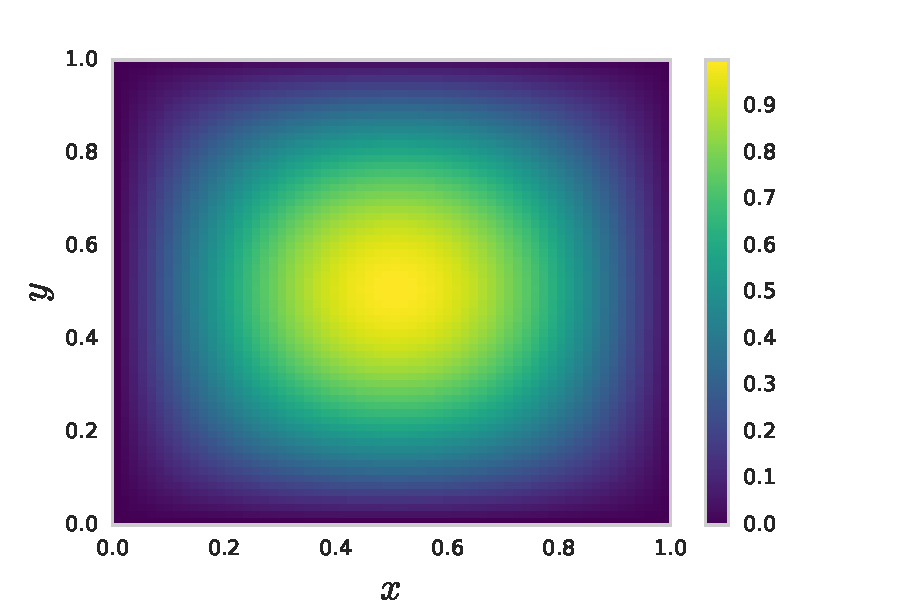
\includegraphics[width=1\linewidth]{figures/twod-deterministic-approx.pdf}
    \end{subfigure}
    \caption{Heatmap plots of the exact solution $u(\v{x})$ (top) against
             $u^h(\v{x})$ (bottom) with $N = 64$ in the case
             $a = 1, \v{b} = \v{0}, c = 0$}
    \label{fig:twod-deterministic-exact-v-approx}
\end{figure}

\begin{figure}
    \centering
    \includegraphics[width=0.75\linewidth]{figures/twod-deterministic-errors.pdf}
    \caption{Plot of $|| u - u^h ||_2$ for various values of  $N$}
    \label{fig:twod-deterministic-error}
\end{figure}
